\documentclass[11pt]{article}

\usepackage{ctex}
\usepackage{amsmath, amssymb}
\usepackage{graphicx}
\usepackage{booktabs}
\usepackage{geometry}
\usepackage{float}
\usepackage{bm}

\geometry{a4paper, margin=2.5cm}
\graphicspath{{figures/}}

\begin{document}

\section{高斯混合分布与参数估计}

按题目给定的二维三成分高斯混合分布
$p(\mathbf{x}) = \sum_{k=1}^{3} \pi_k \mathcal{N}(\mathbf{x}; \bm{\mu}_k, \bm{\Sigma}_k)$
采样 $N = 1000$ 个样本（随机种子固定为 $42$）。其中成分 2（中心 $(3,0)$）与成分 3
（中心 $(2,2)$）部分重叠，是聚类与密度估计中较难处理的区域。图~\ref{fig:true} 给出
真实混合密度，作为后续非参数估计的对照基准。

\begin{figure}[H]
    \centering
    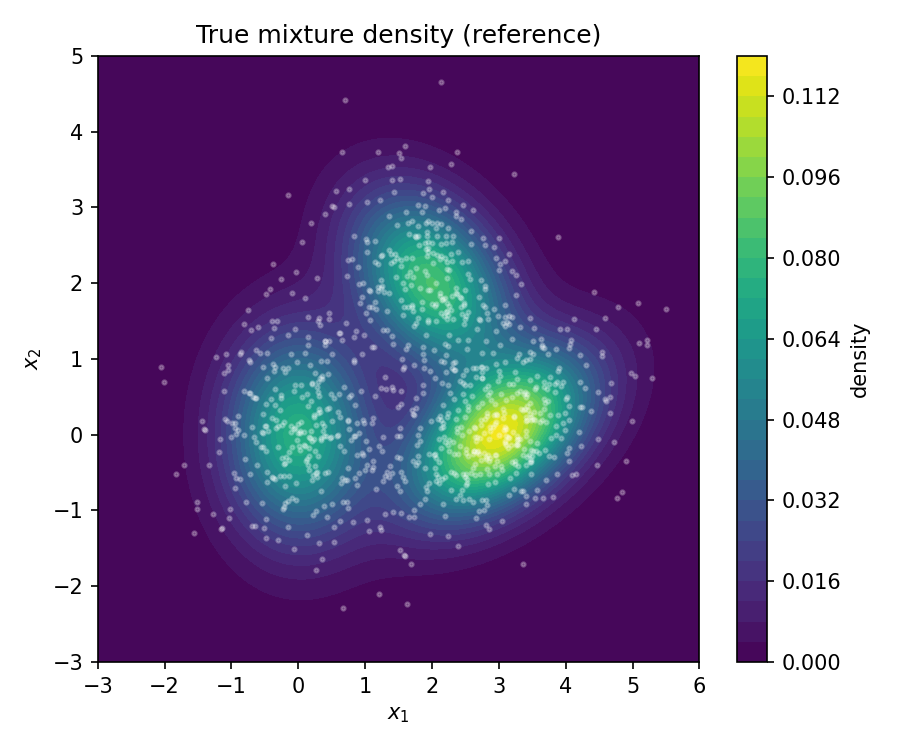
\includegraphics[width=0.55\textwidth]{true_density.png}
    \caption{真实混合密度（参考基准），白点为 $1000$ 个样本。}
    \label{fig:true}
\end{figure}

\subsection{EM 算法估计 GMM 参数}

设聚类数 $K = 3$。初始化时混合系数取均匀分布 $\pi_k = 1/K$，均值取随机样本点，协方差
取全体样本协方差。E 步计算责任度
\[
\gamma_{nk} = \frac{\pi_k \mathcal{N}(\mathbf{x}_n; \bm{\mu}_k, \bm{\Sigma}_k)}
                   {\sum_{j} \pi_j \mathcal{N}(\mathbf{x}_n; \bm{\mu}_j, \bm{\Sigma}_j)};
\]
M 步记 $N_k = \sum_n \gamma_{nk}$，更新
$\pi_k = N_k/N$，$\bm{\mu}_k = \frac{1}{N_k}\sum_n \gamma_{nk}\mathbf{x}_n$，
$\bm{\Sigma}_k = \frac{1}{N_k}\sum_n \gamma_{nk}(\mathbf{x}_n-\bm{\mu}_k)(\mathbf{x}_n-\bm{\mu}_k)^\top$。
协方差每次更新后加 $10^{-6}\mathbf{I}$ 防奇异，以相邻对数似然增量 $<10^{-5}$ 为收敛判据。

本次实验在 $54$ 次迭代后收敛，对数似然 $-3179.12$，曲线单调上升（图~\ref{fig:ll}），
与 EM 保证似然不下降的理论一致。按均值最近距离将估计成分与真实成分匹配后，参数对比
见表~\ref{tab:cmp}：混合系数误差 $\le 0.018$，均值 $L_2$ 误差 $\le 0.16$，协方差
Frobenius 误差在 $0.06\sim0.13$，误差小且主要来自有限采样。图~\ref{fig:em} 中估计
等高线（红实线）与真实等高线（黑虚线）几乎重合，即使在成分 2、3 交叠处，EM 也能借助
协方差形状（成分 2 正相关、成分 3 负相关）正确分开两类，体现了 GMM 软聚类对非球形、
重叠簇的适应能力。

\begin{figure}[H]
    \centering
    \begin{minipage}{0.4\textwidth}
        \centering
        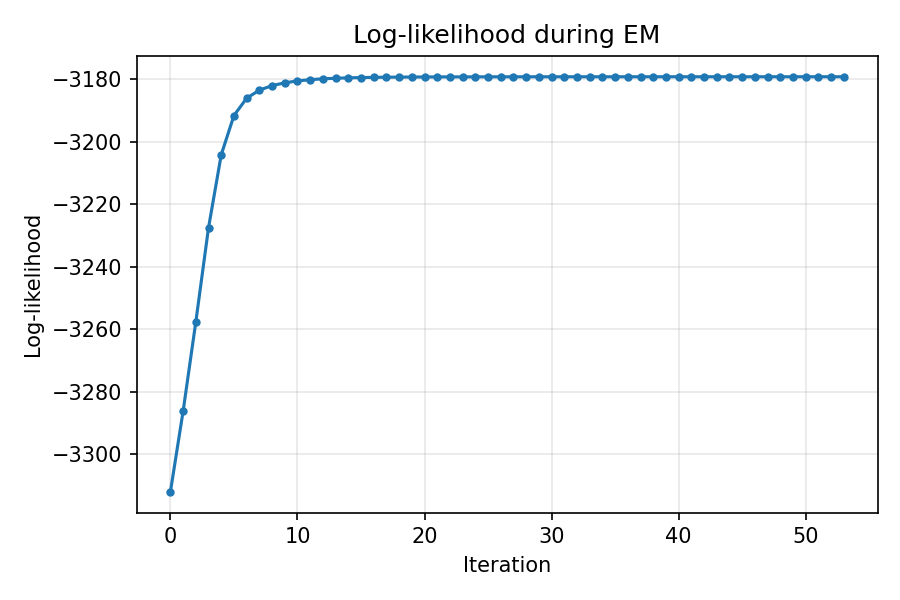
\includegraphics[width=\textwidth]{em_loglikelihood.png}
        \caption{对数似然曲线。}
        \label{fig:ll}
    \end{minipage}\hfill
    \begin{minipage}{0.56\textwidth}
        \centering
        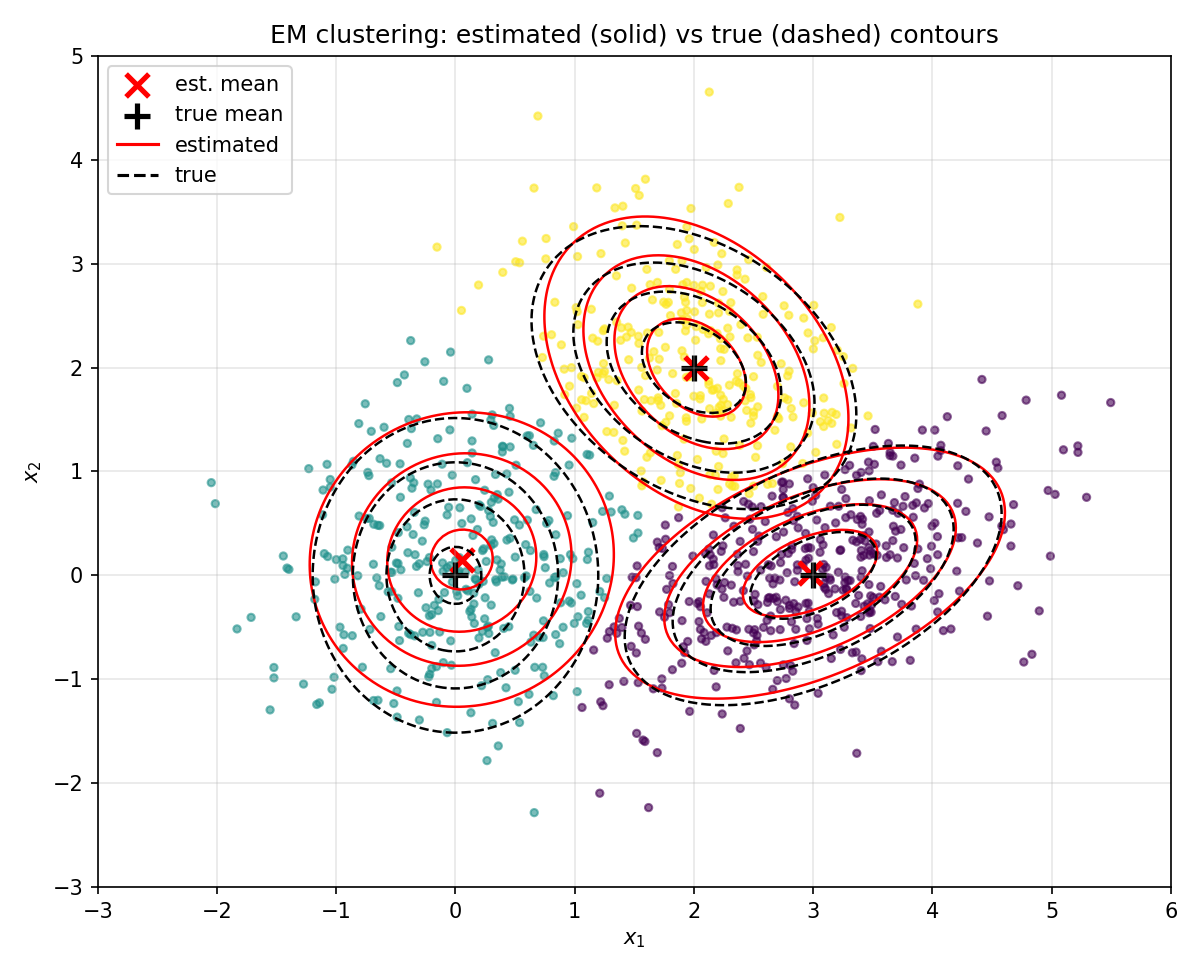
\includegraphics[width=\textwidth]{em_clustering.png}
        \caption{聚类结果：红实线为估计、黑虚线为真实等高线。}
        \label{fig:em}
    \end{minipage}
\end{figure}

\begin{table}[H]
    \centering
    \caption{估计参数与真实参数对比（已按均值匹配）}
    \label{tab:cmp}
    \begin{tabular}{llll}
        \toprule
         & 成分 1 & 成分 2 & 成分 3 \\
        \midrule
        $\pi$ 真实 / 估计 & $0.30 / 0.318$ & $0.40 / 0.389$ & $0.30 / 0.293$ \\
        $\bm{\mu}$ 真实   & $(0,0)$ & $(3,0)$ & $(2,2)$ \\
        $\bm{\mu}$ 估计   & $(0.05,0.15)$ & $(2.97,0.02)$ & $(2.02,2.00)$ \\
        $\bm{\mu}$ 的 $L_2$ 误差 & $0.161$ & $0.034$ & $0.021$ \\
        $\bm{\Sigma}$ 的 Frobenius 误差 & $0.126$ & $0.061$ & $0.112$ \\
        \bottomrule
    \end{tabular}
\end{table}

\subsection{三种非参数密度估计}

基于同样的 $1000$ 个样本，分别用直方图、高斯核（KDE）、$K$ 近邻估计密度，并改变各自的
平滑参数，均与图~\ref{fig:true} 的真实密度对照。

\paragraph{直方图。} 将平面划分为 $\text{bins}\times\text{bins}$ 等距网格，统计样本
比例除以格子面积。图~\ref{fig:hist}：$\text{bins}=10$ 过宽，三个峰糊成一片（偏差大）；
$\text{bins}=40$ 过窄，空格子与孤立尖峰多（方差大）；$\text{bins}=20$ 最接近真实密度。

\begin{figure}[H]
    \centering
    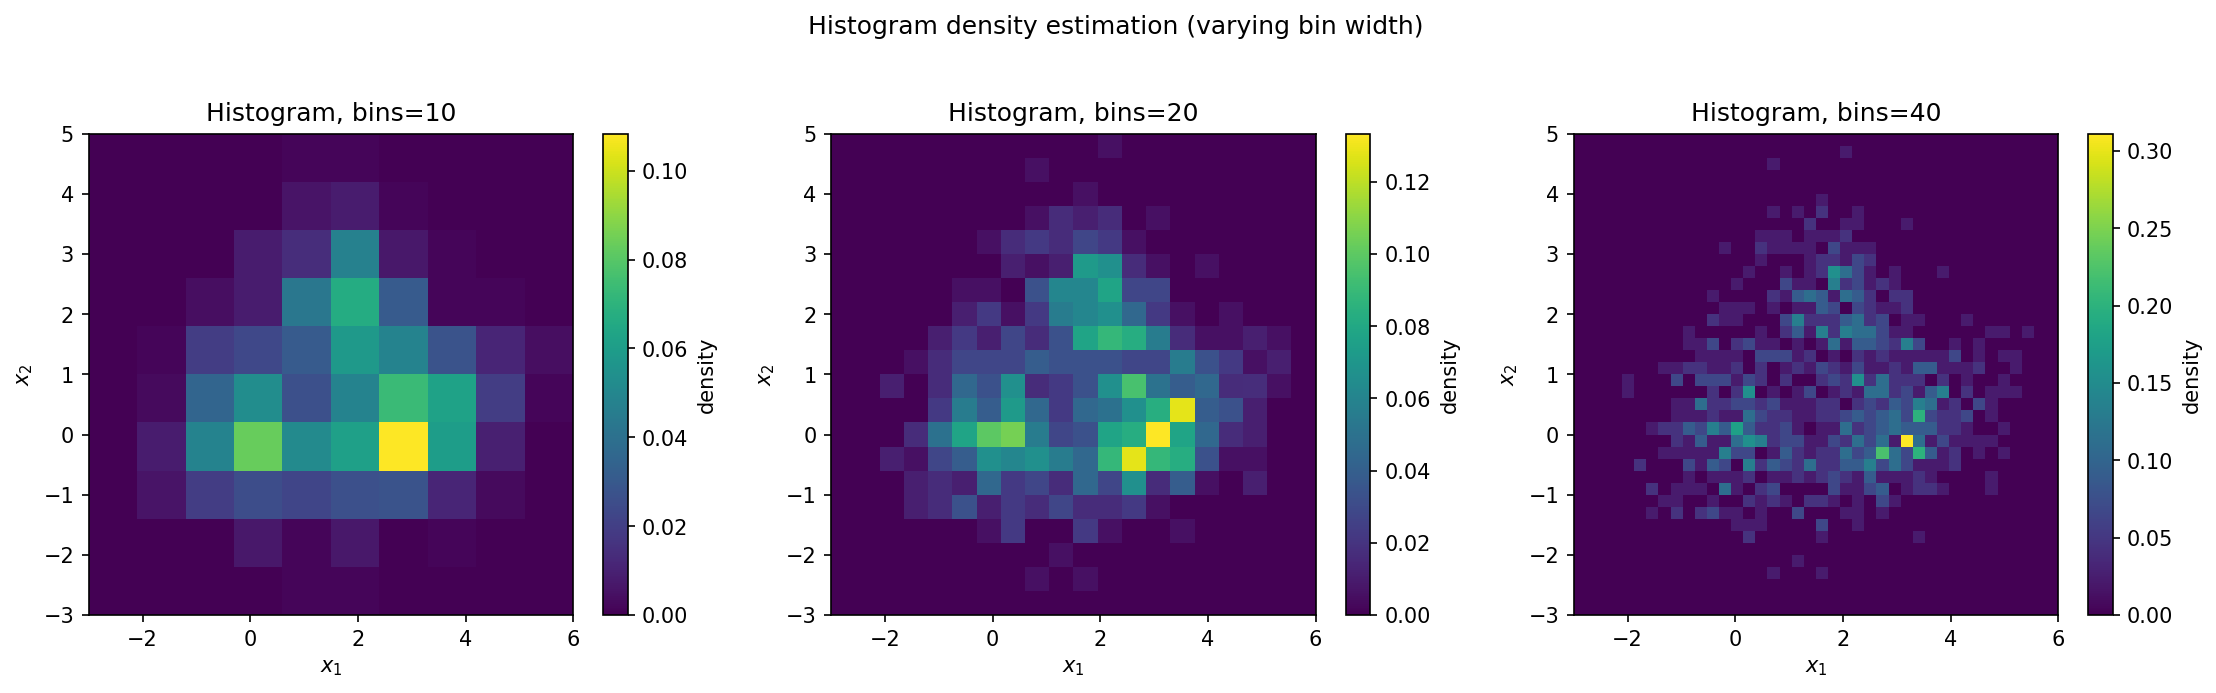
\includegraphics[width=\textwidth]{hist_density.png}
    \caption{直方图密度估计，bin 数取 $10$、$20$、$40$。}
    \label{fig:hist}
\end{figure}

\paragraph{高斯核密度估计。} 用各向同性高斯核，带宽方差 $H^2$：
$\hat{p}(\mathbf{x}) = \frac{1}{N}\sum_n \frac{1}{2\pi H^2}
\exp(-\|\mathbf{x}-\mathbf{x}_n\|^2 / 2H^2)$。图~\ref{fig:kde}：$H^2=0.05$ 欠平滑、
小尖峰多；$H^2=0.8$ 过平滑、三峰并成一团；$H^2=0.2$ 适中、最接近真实密度。相比直方图，
KDE 连续光滑且不依赖网格边界。

\begin{figure}[H]
    \centering
    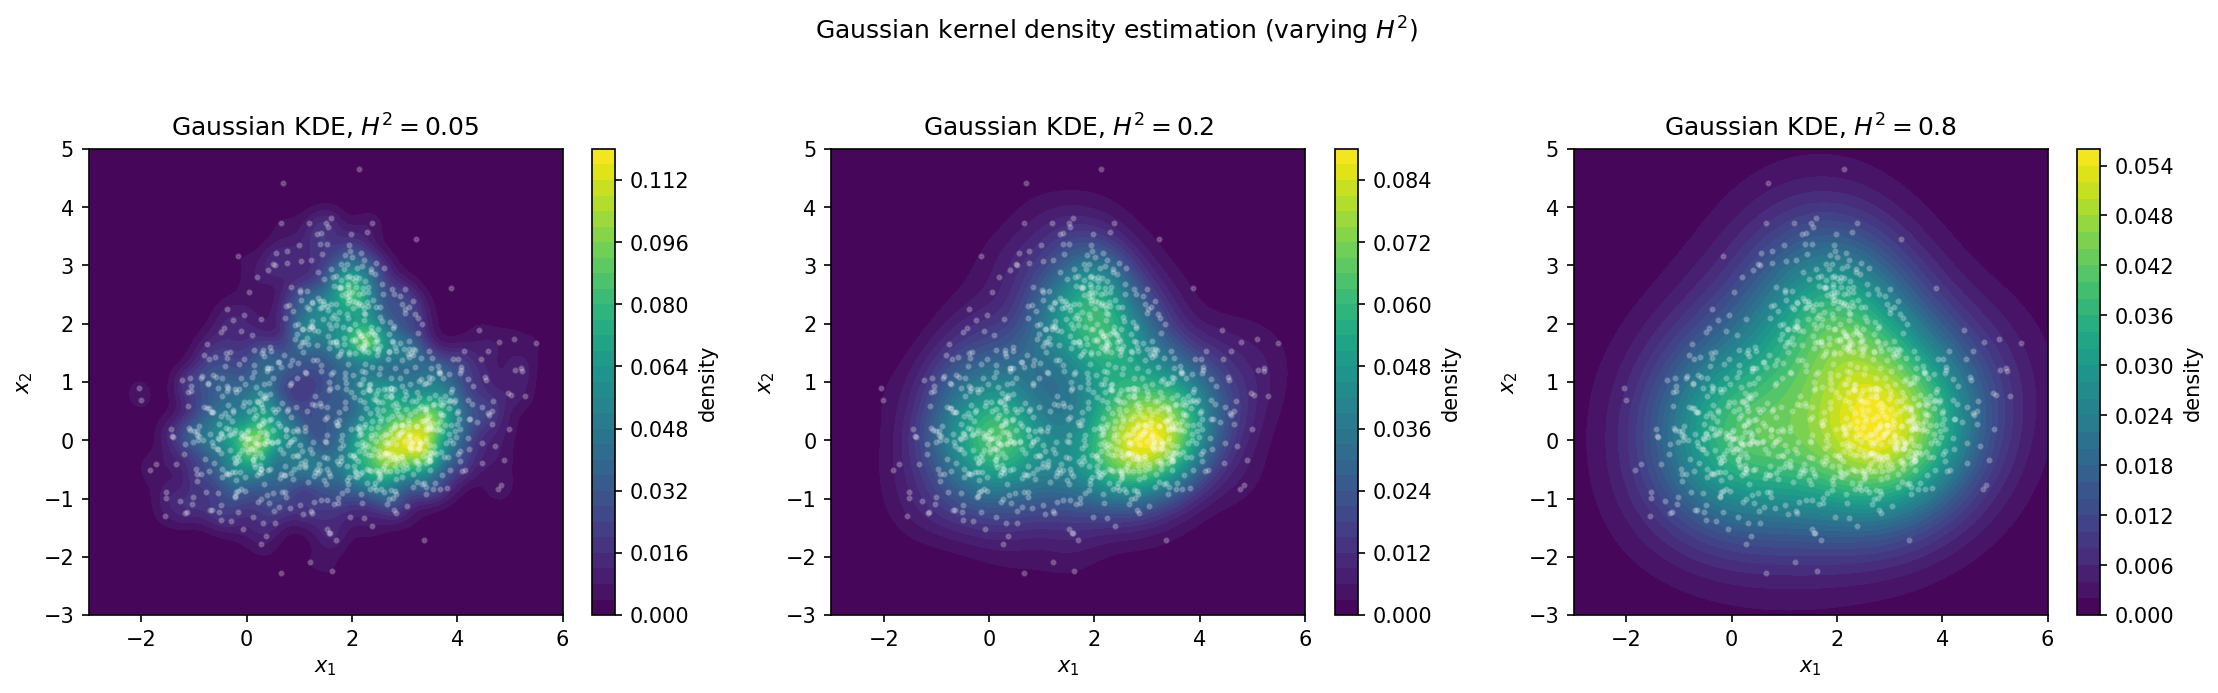
\includegraphics[width=\textwidth]{kde_density.png}
    \caption{高斯核密度估计，核方差 $H^2$ 取 $0.05$、$0.2$、$0.8$。}
    \label{fig:kde}
\end{figure}

\paragraph{$K$ 近邻密度估计。} 以第 $K$ 近邻距离 $r_K$ 的覆盖面积 $\pi r_K^2$ 估计密度：
$\hat{p}(\mathbf{x}) = K / (N \pi r_K^2)$。图~\ref{fig:knn}：$K=5$ 噪声大、虚假结构多；
$K=50$ 过平滑、峰形模糊；$K=20$ 较均衡。该方法带宽自适应（密集区分辨率高、稀疏区自动
加大平滑），但密度不可积，尾部随距离缓慢衰减导致边缘区域被系统性高估（$K=50$ 尤为明显）。

\begin{figure}[H]
    \centering
    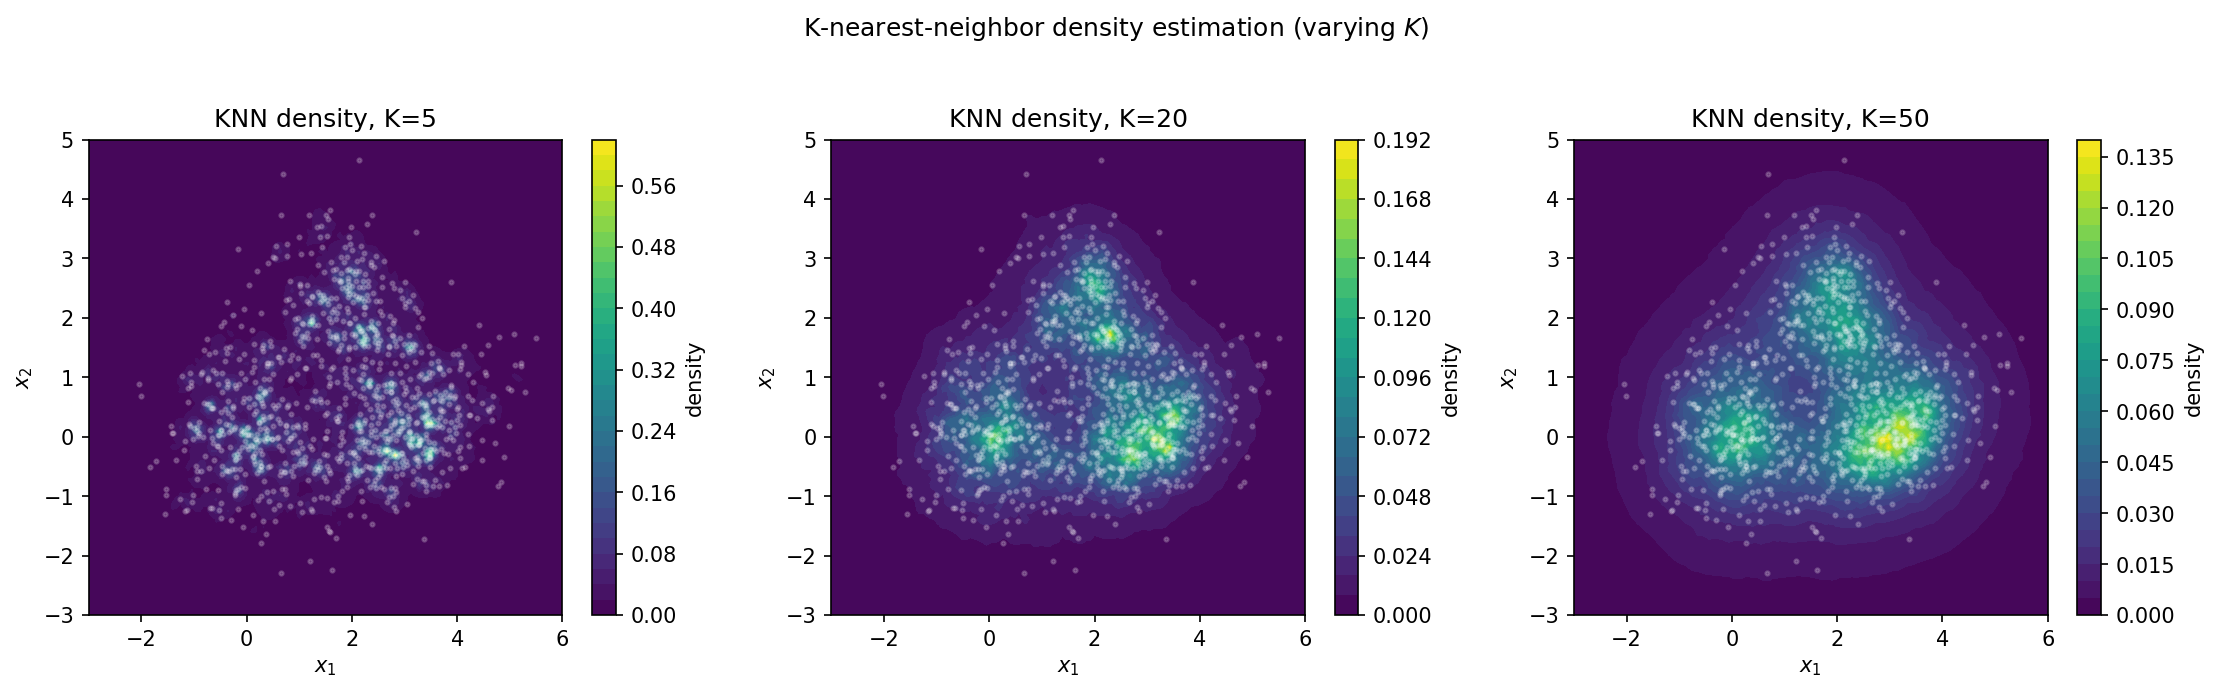
\includegraphics[width=\textwidth]{knn_density.png}
    \caption{$K$ 近邻密度估计，近邻数 $K$ 取 $5$、$20$、$50$。}
    \label{fig:knn}
\end{figure}

三种方法各有一个控制偏差—方差权衡的平滑参数（bin 宽度、$H^2$、$K$）：过小则欠平滑、
噪声大，过大则过平滑、丢结构，取适中值才能较好还原真实密度。综合来看，高斯 KDE
（$H^2=0.2$）最接近真实密度；直方图最简单但不连续；$K$ 近邻带宽自适应但密度不可积、
尾部偏高。

\end{document}
